\label{sec:implUi}
The User Interface (UI) for \emph{rmt}'s home page, seen in figure \ref{fig:rmtCurrent}, was based largely on the refined design seen in figure \ref{fig:refinedDesign}, so each host is assigned to a tower, represented by a Bootstrap panel, each with a different colour representing the colours of the physical towers seen in figure \ref{fig:pitowers}.
This parallel with the real world means that it is intuitive to understand which hosts belong to which tower.

There are minor differences between the finished product and the design in that the large header is removed in favour of a more conservative and Bootstrap-friendly header in the top left of the page.
This also provides the main link to the home page from any other page which many other websites employ (such as reddit \citep{reddit}, University of Glasgow's website \citep{glaWebsite}, and YouTube \citep{youtube}) in a similar fashion.

Adding hosts is no longer on the home page to make room for more hosts and because adding a host is not such a common operation that it needs to be on the home page.
In the case of PiCloud the add host form should be used to add the hosts to their corresponding towers and then left alone indefinitely until more Raspberry Pis are added to the PiCloud for example.
So instead of having the form on the home page, the form is on a separate page accessed by the plus icon in the top left of the home page.

Next to this are links to the PiCloud website, since they were the ones to request the creation of this software, and a link to the GitHub page of \emph{rmt} since, as previously stated, the project will be made open source, and this provides an easy way for the user to find, and potentially contribute to, the project.

\begin{figure}[t]
	\centering
	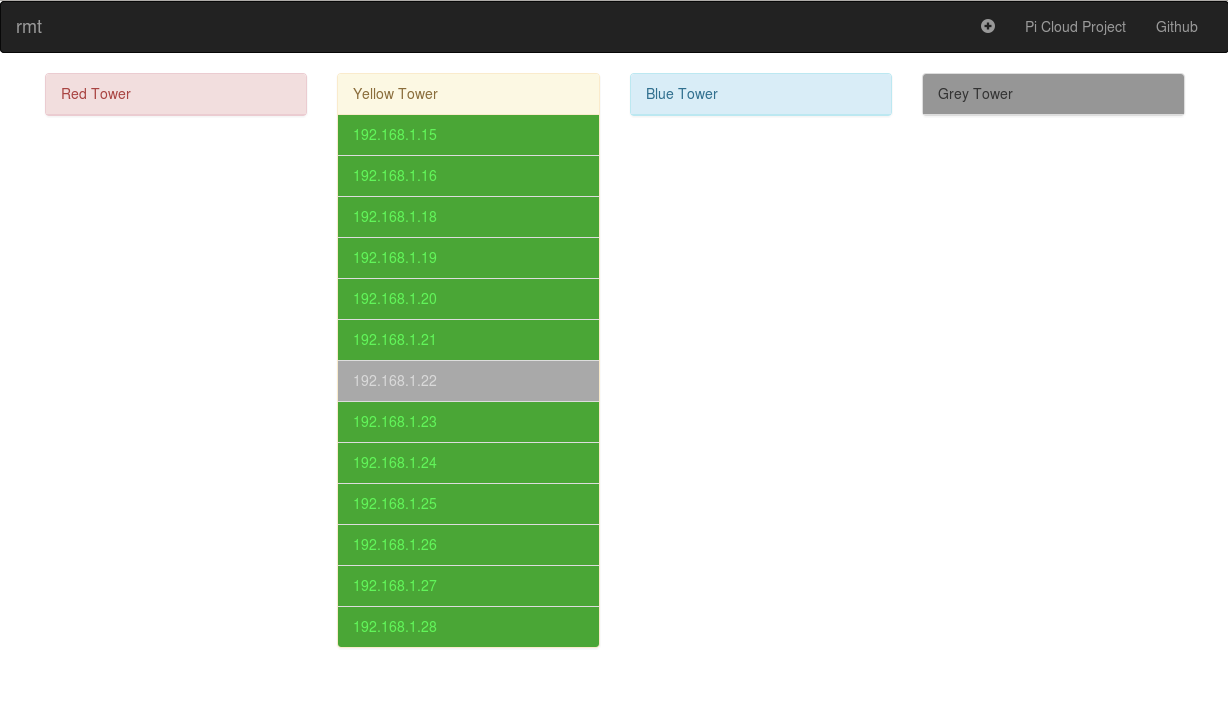
\includegraphics[width=0.8\textwidth]{rmtCurrent}
	\caption{\emph{rmt}: home page}
	\label{fig:rmtCurrent}
\end{figure}

\begin{figure}[t]
	\centering
	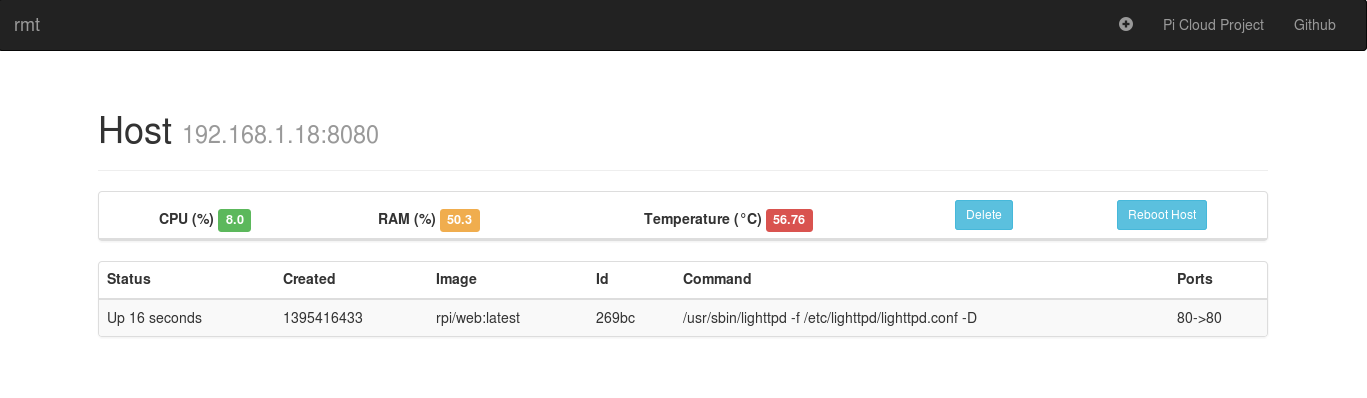
\includegraphics[width=0.8\textwidth]{rmtHostsCurrent}
	\caption{\emph{rmt}: host page}
	\label{fig:rmtHostCurrent}
\end{figure}

The design of the hosts page is somewhat inspired by the interface of Shipyard
